
\documentclass[preview]{standalone}
\usepackage{times}            % Font choice
\usepackage{amsmath}          % AMS
\usepackage{amssymb}          % AMS
\usepackage[OT2,T1]{fontenc}  % Cyrillic and standard % TODO: make alphabet options more general
\usepackage[utf8]{inputenc}   % UTF-8 support
\usepackage{fancyhdr}         % Headers
\usepackage{graphicx}         % Graphics
\usepackage{wrapfig}          % Illustrations
\usepackage{import}           % Proper file inclusion
\usepackage{caption}
\usepackage{subcaption}
\usepackage{fancyvrb}         %
\usepackage{listingsutf8}     % For samples
\usepackage[left=1in,right=1in,top=0.75in,bottom=0.75in]{geometry}
%\usepackage{fullpage}        % Set up margins for full page
\usepackage{url}              % Urls
\usepackage[normalem]{ulem}   % \sout

\begin{document}

\begin{figure}
\centering
\begin{minipage}[t]{.5\textwidth}
  \strut\vspace*{-\baselineskip}\newline
  \centering
  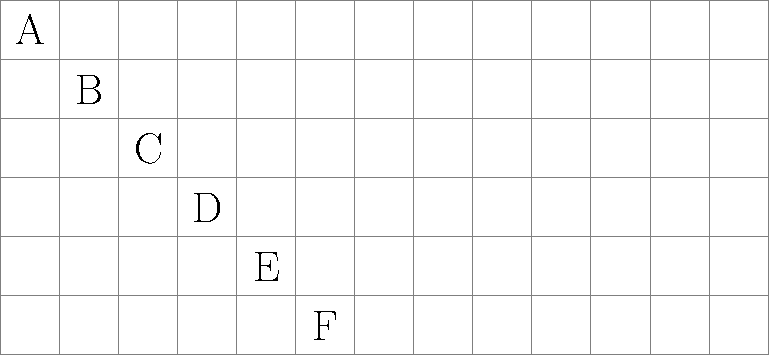
\includegraphics[width=.8\linewidth]{grid1.pdf}
  \captionsetup[figure]{width=.8\linewidth,justification=centering,labelformat=empty}
  \captionof{figure}{Efter 6 bokstäver är skrivna}
  \label{fig:test1}
\end{minipage}%
\begin{minipage}[t]{.5\textwidth}
  \strut\vspace*{-\baselineskip}\newline
  \centering
  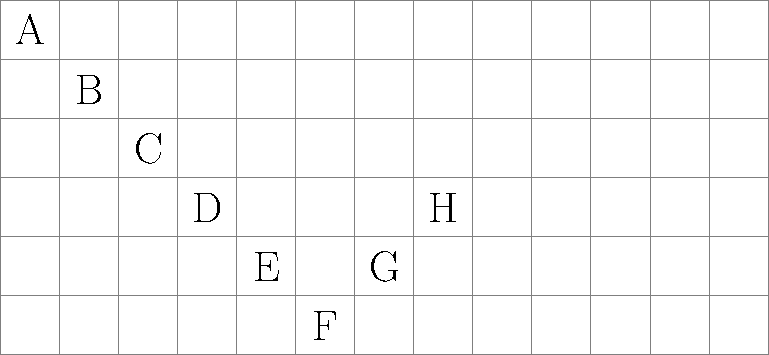
\includegraphics[width=.8\linewidth]{grid2.pdf}
  \captionsetup[figure]{width=.8\linewidth,justification=centering,labelformat=empty}
  \captionof{figure}{Efter 8 bokstäver är skrivna, vi har nu studsat en gång i bottenväggen}
  \label{fig:test2}
\end{minipage}
\end{figure}
\begin{figure}[!h]
\centering
\begin{minipage}[t]{.5\textwidth}
  \centering
  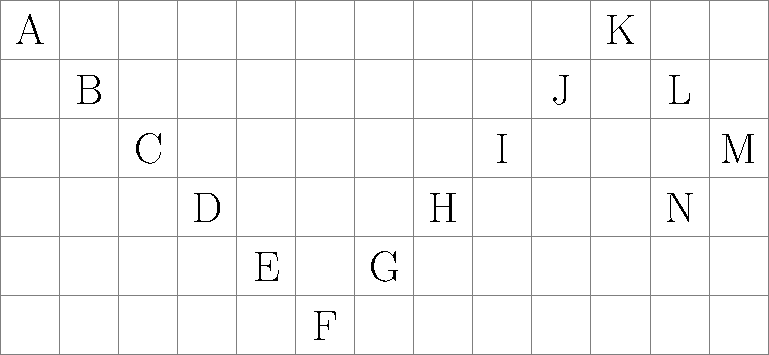
\includegraphics[width=.8\linewidth]{grid3.pdf}
  \captionsetup[figure]{width=.8\linewidth,justification=centering,labelformat=empty}
  \captionof{figure}{Efter 14 bostäver är skrivna, vi har nu även
studsat i övre och högra väggen}
  \label{fig:test1}
\end{minipage}%
\begin{minipage}[t]{.5\textwidth}
  \centering
  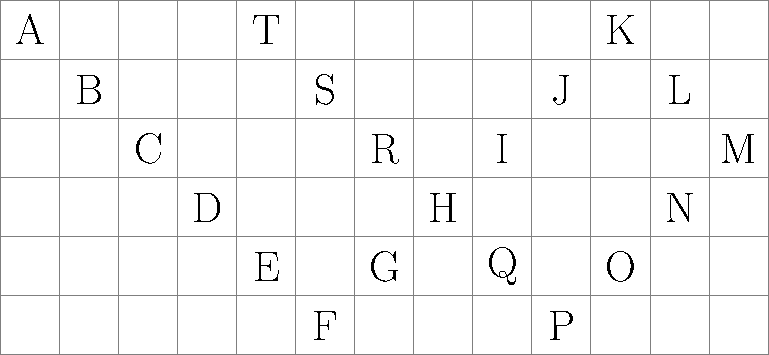
\includegraphics[width=.8\linewidth]{grid4.pdf}
  \captionsetup[figure]{width=.8\linewidth,justification=centering,labelformat=empty}
  \captionof{figure}{Efter alla $20$ bokstäver är skrivna, notera att vi inte skrev över \texttt{H}:et med ett \texttt{R}, utan vi skrev \texttt{R}:et på nästa lediga plats}
  \label{fig:test2}
\end{minipage}
\end{figure}

\end{document}

